\documentclass[10pt]{article}
\usepackage[pdftex]{graphicx}
\graphicspath{{./images/}}
\usepackage{amsmath,amssymb}
\usepackage{dirtytalk}
\usepackage{anyfontsize}
\usepackage{xcolor}
\usepackage{hyperref}
\hypersetup{
    colorlinks,
    linkcolor={red!50!black},
    citecolor={blue!50!black},
    urlcolor={blue!80!black}
}
\usepackage[skip=10pt plus1pt, indent=40pt]{parskip}
\usepackage{../common_styles/csagh}


\begin{document}
\begin{opening}
  \title{Decision trees with Python}
  \author[Universidad Autónoma de Nuevo León, San Nicolás de los Garza, aldo.hernandezt@uanl.edu.mx]{Aldo Hernández}

  \keywords{...}
  \begin{abstract}
    This document explores decision tree algorithms for classification tasks, focusing on Boolean classification where inputs have discrete values and outputs have two possible values. The document explains how decision trees function through sequential tests at each node, with branches representing attribute values and leaf nodes providing final decisions. It discusses the challenges of representing all Boolean functions efficiently and the exponential growth of possible functions as attributes increase. The methodology section details a practical implementation using a dataset of songs, predicting whether they reached the top position on Billboard charts. The process includes data preprocessing to handle missing values, mapping categorical variables to numerical ones, and determining optimal tree depth through k-fold cross-validation. The resulting decision tree achieves 71.18\% accuracy and successfully predicts that Camila Cabello's "Havana" would reach number one. The paper concludes that decision trees are powerful classification models that perform best with large, complete datasets, though they require careful handling of categorical and continuous variables. Through thorough preliminary analysis, the implemented model demonstrates reliable predictive capability for music chart performance.
  \end{abstract}

  \keywords{decision tree, machine learning, python, cross-validation}
\end{opening}

\section{Introduction}
A decision tree is a function that takes as input a vector of attribute values and returns a single output value---also called decision---. The input and output values can be discrete or continuous \cite{ai}. When inputs have discrete values and the output has exactly two possible values it is called a \textbf{Boolean classification}, since any example input will be classified as true or false. \par
For the decision tree to reach a decision, it has to perform a sequence of tests. Each tree node corresponds to a test of the value of one of the input attributes ($A_{i}$), and the branches from the node are labeled with the possible values for said attributes ($A_{i} = v_{ik}$). Each \textit{leaf node} specifies a value to be returned by the function \cite{ai}. \par
This representation is very common for humans; for example, when there is a high rain probability and the question "should I take an umbrella?" arises, how we decide to take it or not is essentially a decision tree. These decisions are of the type "if this, then that" \cite{aprendeML}. \par
A Boolean decision tree is logically equivalent to the assertion that the goal attribute is true if and only if the input attributes satisfy one of the paths leading to a leaf with value \textit{true} \cite{ai} \par
\begin{equation*}
    Goal \Leftrightarrow (Path_{1} \vee Path_{2} \vee \dots)
\end{equation*}
\begin{equation*}
    Path_{i} = (A_{i} = v_{ik} \wedge A_{j} = v_{jk} \wedge \dots)
\end{equation*}
For a wide variety of problems, the decision tree format has a nice concise result. But some functions cannot be represented concisely. So decision trees are good for some kinds of functions and bad for others. Now, consider the set of all Boolean functions on $n$ attributes, how many different functions are in this set? The answer is basically how many different true tables can be written down since the function is defined by its truth table. A truth table over $n$ attributes has $2^{n}$ rows (one for each combination of attributes). The "answer" column of the truth table can be considered as a $2^{n}$-bit number that defines the function, which means that there are $2^{2^{n}}$ different functions since each function has a version that outputs \textit{true} for that specific $2^{n}$-bit number and another version that outputs \textit{false} for the same number. The reader can see that this number gets exponentially big as we have more and more attributes, and we will have an even larger number of possible trees to choose from since multiple trees can compute the same function. So it is impossible to find \textit{any} kind of representation that is efficient for \textit{all} kinds of functions. \cite{ai} \par
For this algorithm, it may seem obvious that we want a tree that is consistent with the examples and is as small as possible. But because of what was stated above, there is no efficient way to search through the more than $2^{2^{n}}$ trees for the tree that we want. However, with some heuristics it is possible to find a good approximate solution: a small consistent tree. The \textbf{decision-tree-learning} algorithm adopts a \textbf{greedy divide-and-conquer} strategy: always test the most important---the one that makes the most difference when classifying---attribute first \cite{ai}. This test divides the problem up into smaller subproblems that can be then solved recursively. \par
After the first attribute test splits up the examples, each outcome is a new decision tree learning problem in itself, there are four cases to consider for these recursive problems:
\begin{itemize}
    \item If the remaining examples are all positive or all negative, the decision can be done.
    \item If there are some positive and some negative examples, then choose the best attribute to split them.
    \item If there are no examples left, no example has been observed for this combination of values, so we return a default value.
    \item If there are no attributes left, but both positive and negative examples, it means that said examples have the exact same description, but different classifications. This can happen because there is an error or \textbf{noise} in the data; because the domain is nondeterministic; or because we couldn't observe an attribute that would distinguish the examples. The best we can do is to return the most frequent type of the remaining examples, i. e. if you have left 3 positives and 2 negatives, return positive.
\end{itemize}
It is important to note that this algorithm does not look at the \textit{correct} Boolean functions, instead, it looks at the given examples to draw a simple small-fitting tree that is consistent with all the examples. \par
The accuracy of a learning algorithm can be evaluated with a \textbf{learning curve}. For a decision tree in a problem domain, the curve shows that as the training set size grows, accuracy increases \cite{ai}. \par
The greedy search used in this type of learning is designed to minimize the depth of the final tree, the idea is to pick the attribute that goes as far as possible towards providing an exact classification of the examples. A perfect attribute will divide the examples into sets that area all positive or all negative---and thus, be leaves of the tree---\cite{ai}. Now, the question arises, how can we measure this? For that, we will use the notion of information gain, defined in terms of \textbf{entropy}. \par
Entropy is a measure of the uncertainty of a random variable; acquisition of information corresponds to a reduction in entropy \cite{ai}. In general, the entropy of a random variable $V$ with values $v_{k}$, each with probability $P(v_{k})$ is defined as
\begin{equation*}
    H(V) = \sum_{k}P(V_{k})\log_{2}\left(\frac{1}{P(v_{k})}\right) = - \sum_{k}P(v_{k})\log_{2}P(v_{k})
\end{equation*}
It will help to define $B(q)$ as the entropy of a Boolean random variable that is true with probability $q$:
\begin{equation*}
    B(q) = -(q\log_{2}q + (1-q)\log_{2}(1-q))
\end{equation*}
Going back to decision tree learning, if a training set contains $p$ positive examples and $n$ negative examples, then the entropy of the goal attribute on the whole set is
\begin{equation*}
    H(Goal) = B\left(\frac{p}{p+n}\right)
\end{equation*}
A test on a single attribute $A$ might give us only part of the whole entropy bits of the problem. We can measure exactly how much by looking at the entropy remaining after the attribute test. \par
An attribute $A$ with $d$ different values divides the training set $E$ into subsets $E_{1}, \dots, E_{d}$. Each subset $E_{k}$ has $p_{k}$ positive examples and $n_{k}$ negative examples, so if we go along the $E_{d}$ branch, we will need an additional $B(p_{k}/(p_{k}+n_{k}))$ bits of information to answer the question \cite{ai}. The probability that a randomly selected example from the training set that has the $k$-th value for said attribute is $(p_{k}+n_{k})/(p+n)$, so the expected entropy remaining after testing the attribute $A$ is
\begin{equation*}
    Remainder(A) = \sum_{k=1}^{d}\frac{p_{k}+n_{k}}{p+n}B\left(\frac{p_{k}}{p_{k}+n_{k}}\right)
\end{equation*}
The \textbf{information gain} from the attribute test on $A$ is the expected reduction in entropy: \par
\begin{equation*}
    Gain(A) = B\left(\frac{p}{p+n}\right) - Remainder(A)
\end{equation*} \par
When dealing with continuous values, we may have to use and minimize the \textbf{GINI impurity} index to decide which attribute use next to split the examples, since it will measure how unordered the nodes will be after splitting them up \cite{aprendeML}. However, we will keep focusing only in categorical classification.
On some problems, this algorithm will generate a large tree when there is no pattern to be found since it will seize on any "pattern" it can find in the input. This problem is called \textbf{overfitting} and occurs in all type of learners. Overfitting is more likely as the hypothesis space and number of input attributes grows, and less likely as we increase the number of training examples. \par
For decision trees, there is a technique called \textbf{decision tree pruning} that combats overfitting. It works by eliminating nodes that are not clearly relevant. We start with a full tree generated by decision-tree-learning, then we look at a test node that has \textit{only} leaf nodes as descendants. If the test appears to be irrelevant---detecting only noise in the data---then we eliminate the test replacing it with a leaf node \cite{ai}. \par
But how can we detect a node is testing an irrelevant attribute? If a node were to be irrelevant, we would expect it to split examples into subsets with roughly the same proportion of positive examples as the whole set ($p/(p+n)$) so that the \textit{information gain} will be close to zero. Then, a new question arises, how large should a gain be? \par
For this, we could use a significance test by assuming there is no underlying pattern (null hypothesis). Then, the actual data is analyzed to calculate the extent to which they deviate from a perfect absence of pattern. If the degree of deviation is statistically unlikely (less than 5\% of probability), then it is considered to be good evidence for the presence of a significant pattern in the data. The probabilities are calculated from standard distributions of the amount of deviation one would expect to see in random sampling \cite{ai}. \par
With pruning, noise in examples can be tolerated \cite{ai}. Pruned trees perform significantly better than unpruned trees when the data contains a larga amount of noise. Also, they are often smaller and easier to understand. \par
Another technique is called \textbf{early stopping} and combines pruning with information gain, it consists in having the decision tree algorithm to stop generating nodes when there is no good attribute to split on, instead of generating them all and then pruning them away. The problem with this approach is that it stops us from recognizing situations when there is no good attribute, but there are \textit{combinations} of attributes that are informative. \par
There are several issues with decision trees: 
\begin{itemize}
    \item Missing data: Sometimes, not all attributes values will be known for every example.
    \item Multivalued attributes: When an attribute has many possible values, the information gain measure gives an inappropriate indication of the attribute's usefulness.
    \item Continuous and integer-valued input attributes: They have an infinite set of possible values. Rather than generating infinitely many branches, these algorithms typically find the split point that gives the highest information gain.
    \item Continuous-valued output attributes: When trying to predict a numerical output, we need a regression tree rather than a classification tree. This tree has at each leaf a linear function of some subset of numerical attributes rather than a single value.
\end{itemize}

\newpage
\section{Methodology}
\subsection{Before typing code}
In order to work with our data, we'll need to download the \href{http://www.aprendemachinelearning.com/wp-content/uploads/2018/04/artists_billboard_fix3.csv}{.csv file} \cite{aprendeML} to use it as our dataset along with the \href{https://graphviz.org/download/}{Graph Visualization Software}. Then, we have to make some library imports
\begin{figure}[h]
    \centering
    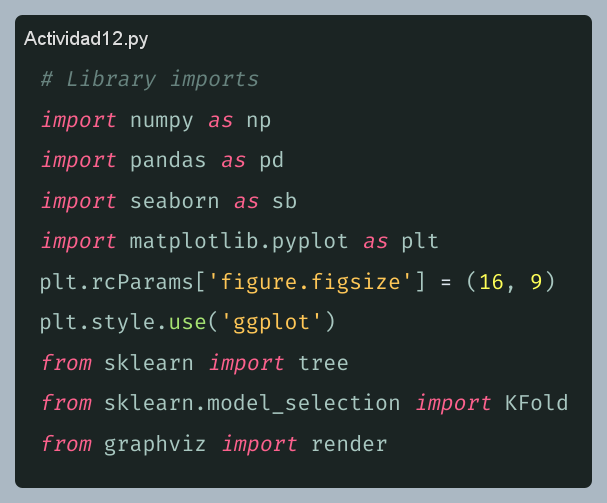
\includegraphics[width=90mm]{2025-03-30-20-00-15.png}
    \caption{Importing libraries.}
\end{figure}

\newpage
\subsection{Initial analysis}
Now, we process the csv file as a Pandas dataset. After that, we see that our data is very unbalanced since we have a lot of songs that did not make the top 1 on billboard charts in comparison to songs that made the top 1. \par
Also, when examining the year of birth of artists, we see that we have a lot of artists that have 0 as their year of birth. This is data that we do not have so we need to fix this in the next subsection.
\begin{figure}[h]
    \centering
    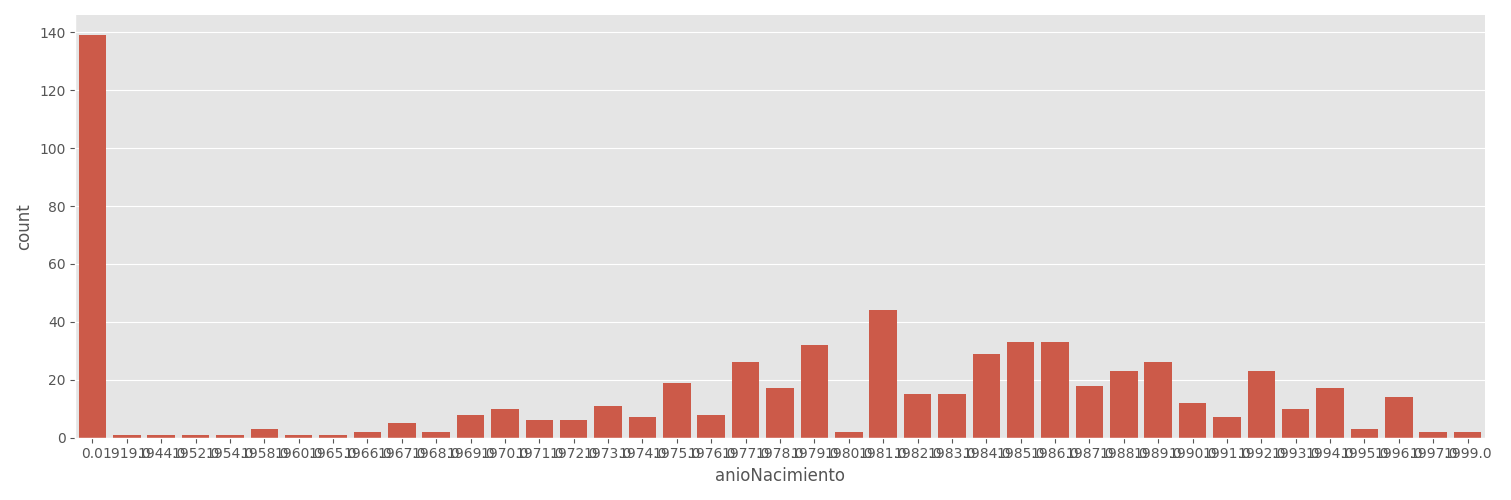
\includegraphics[width=130mm]{year_vs_count.png}
    \caption{Row count per year of birth}
\end{figure}

\subsection{Preparing the data}
The idea behind having a year of birth column is to know the age of the artist at the time they released their song that entered the billboard chart. First, we will replace all zeroes for None with a function that will be applied to the whole dataset. Then, we will use another function to obtain the artist age when the song was released (or None if we don't know the age of the artist). \par
\begin{figure}[h]
    \centering
    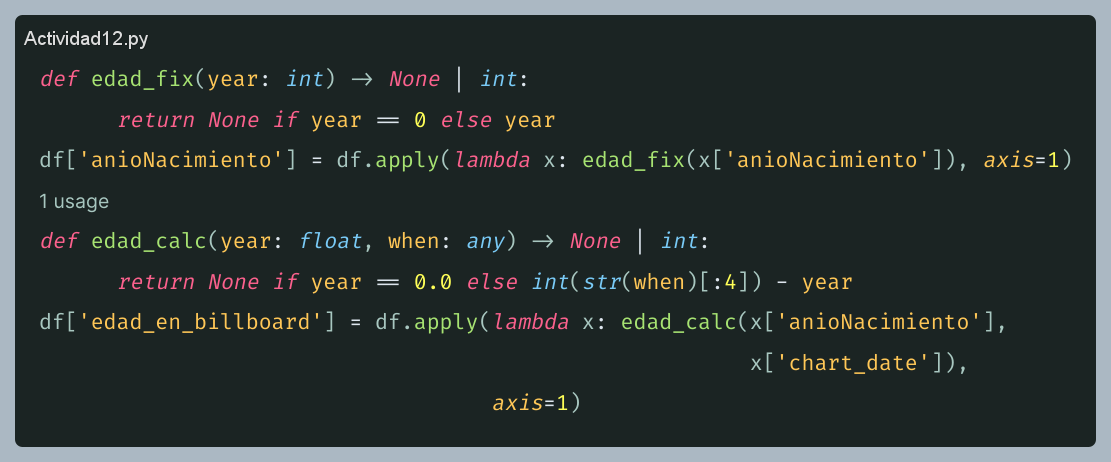
\includegraphics[width=110mm]{2025-03-30-20-56-30.png}
    \caption{Fixing the dataset rows.}
\end{figure}
Next, we will obtain the mean and standard deviation of the ages that we know and generate random numbers within the range of the mean minus deviation to mean plus deviation. This is because statistically the majority of data should be concentrated around these values. \par
\begin{figure}[h]
    \centering
    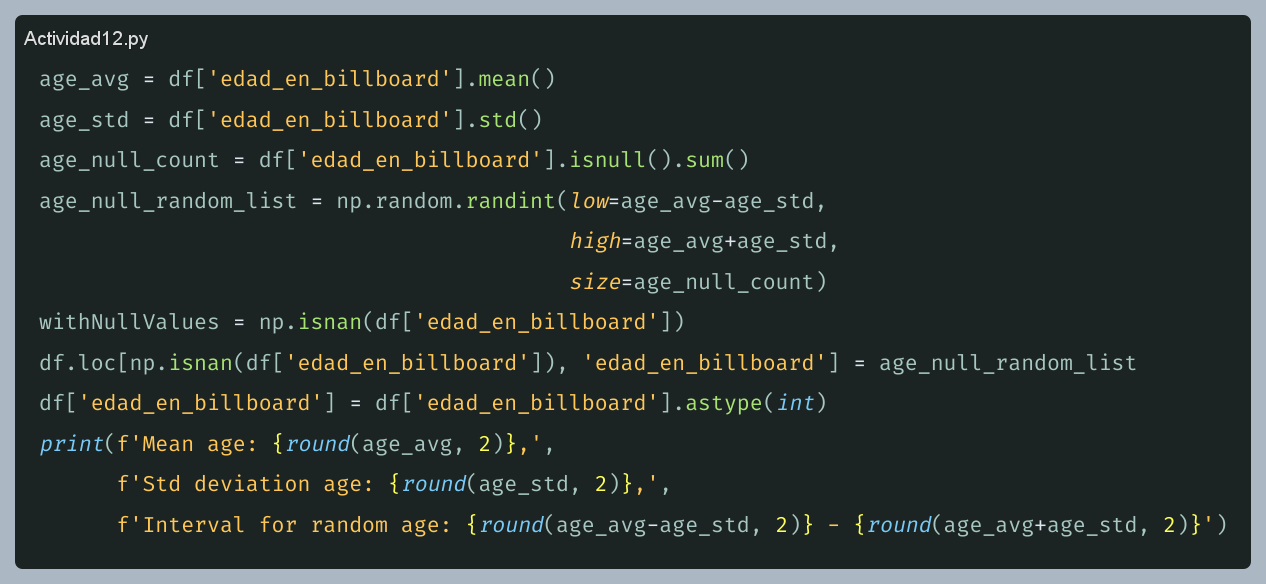
\includegraphics[width=90mm]{2025-03-30-21-00-25.png}
    \caption{Filling unknown ages.}
\end{figure}
We can visualize real values and filled ones in the following plot.
\begin{figure}[h]
    \centering
    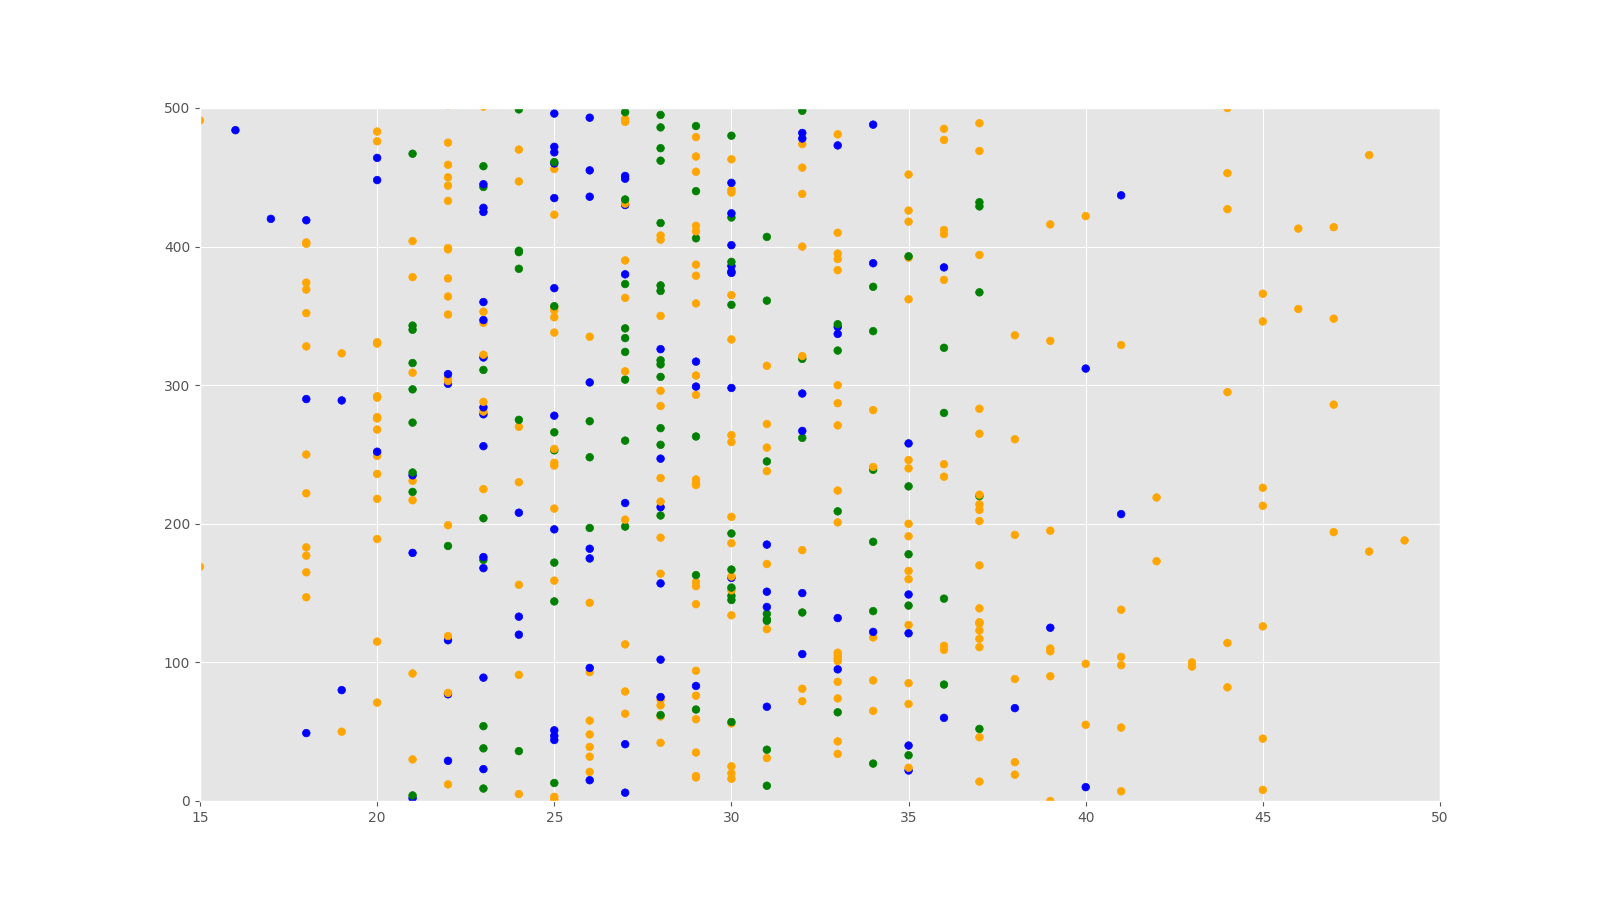
\includegraphics[width=110mm]{age_in_chart_plot.png}
    \caption{Artist age when they released: top 1 songs (blue), no top 1 songs (yellow), and filled year songs (green).}
\end{figure}

\newpage
\subsection{Mapping data}
Another problem with our data is that we have too many categorical variables---such as mood, tempo, genre, and artist type---and continuous variables---like artist age and duration---. To fix this, we have to \textbf{map}---assign a value---each of these categories to a discrete numerical value. Essentially we will then just drop all the old columns since we won't be able to use them for creating our tree.
\begin{figure}[h]
    \centering
    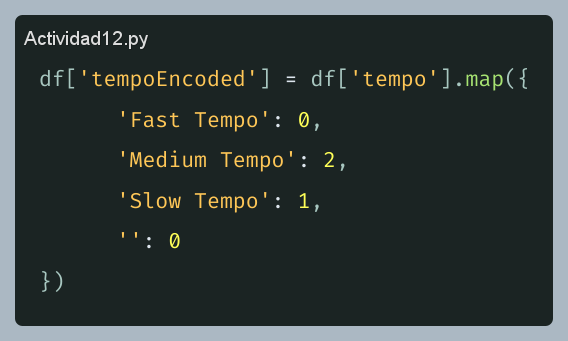
\includegraphics[width=90mm]{2025-03-30-21-14-04.png}
    \caption{Mapping the tempo.}
\end{figure}

\newpage
\subsection{Creating the tree}
To test for model accuracy, we need to test the model on a set of examples it has not seen yet. The first approach to do this is to use \textbf{holdout cross-validation} that consists of randomly splitting the data into a training set that produces the hypothesis $h$ and a validation set that tests the $h$. This approach has a clear disadvantage: it does not use all the available data to get the best hypothesis. A good alternative is to use \textbf{k-fold cross-validation}, the idea of this method is that each example serves as training and test data. First, the data will be split into $k$ equal subsets to then perform $k$ rounds of learning where in each round $1/k$ of the data is used as test set and the remaining examples will be used as training data \cite{ai}. \par
We have to find the most appropriate depth for our tree, for this we will iterate for each possible depth from 1 to 7 (maximum quantity of attributes) creating a tree model with said depth, then using 10-fold cross-validation we will fit and test the model to get an average accuracy. \par
\begin{figure}[h]
    \centering
    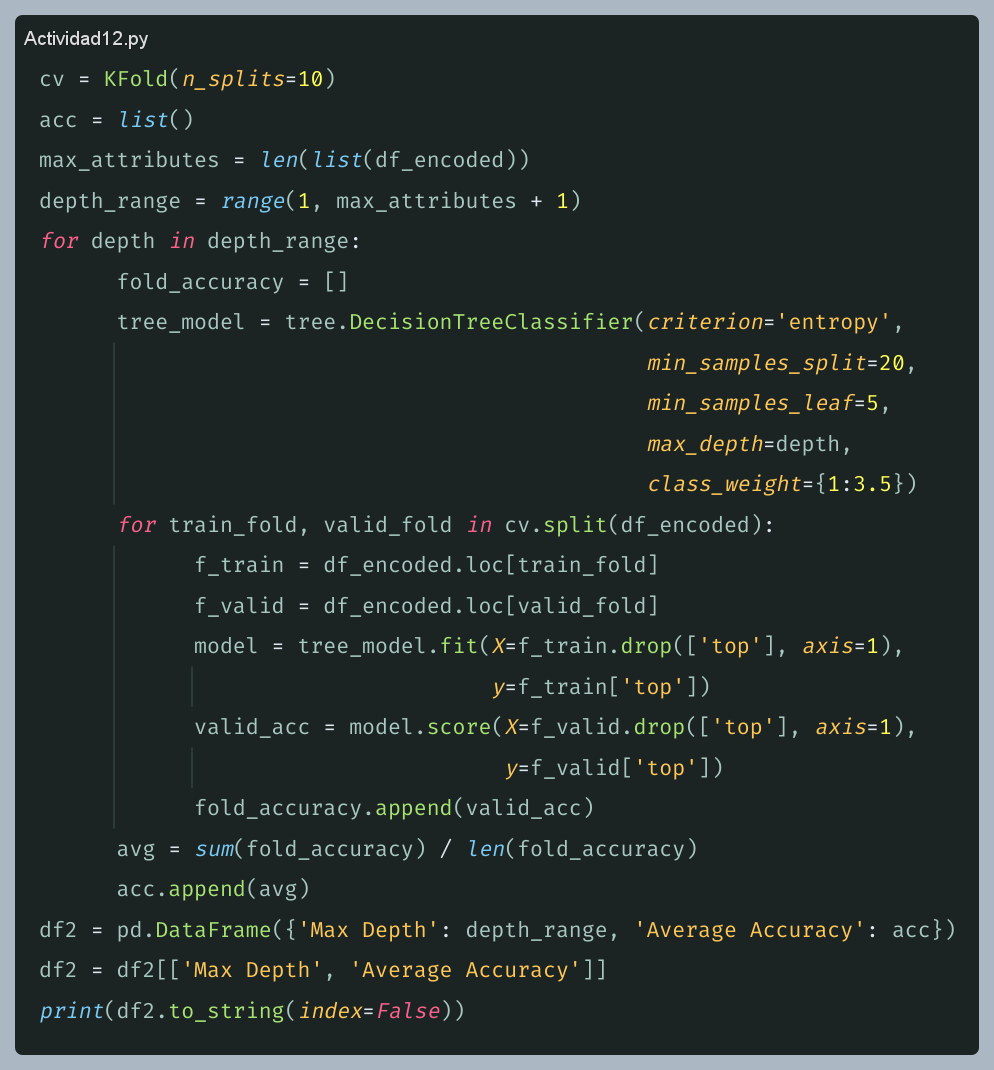
\includegraphics[width=90mm]{2025-03-31-07-38-26.png}
    \caption{Creating models to see the best depth.}
\end{figure}
After doing this, we can see that the highest accuracy in average can be achieved with a depth of 4. Then, we create the tree model and fit it to all our examples, using a class weight ratio of $1:3.5$ since the tree is not balanced (it is the ratio of top 1 songs to no top 1 songs). \par
\begin{figure}[h]
    \centering
    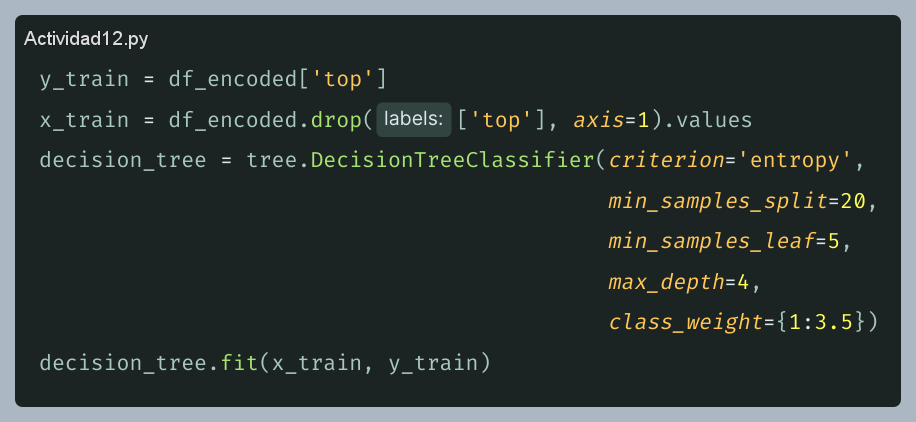
\includegraphics[width=90mm]{2025-03-31-07-47-28.png}
    \caption{Creating the tree with a depth of 4 and class weight.}
\end{figure}
We get a decision tree with an accuracy of $71.18\%$, and we can visualize it in the next figure.
\begin{figure}[h]
    \centering
    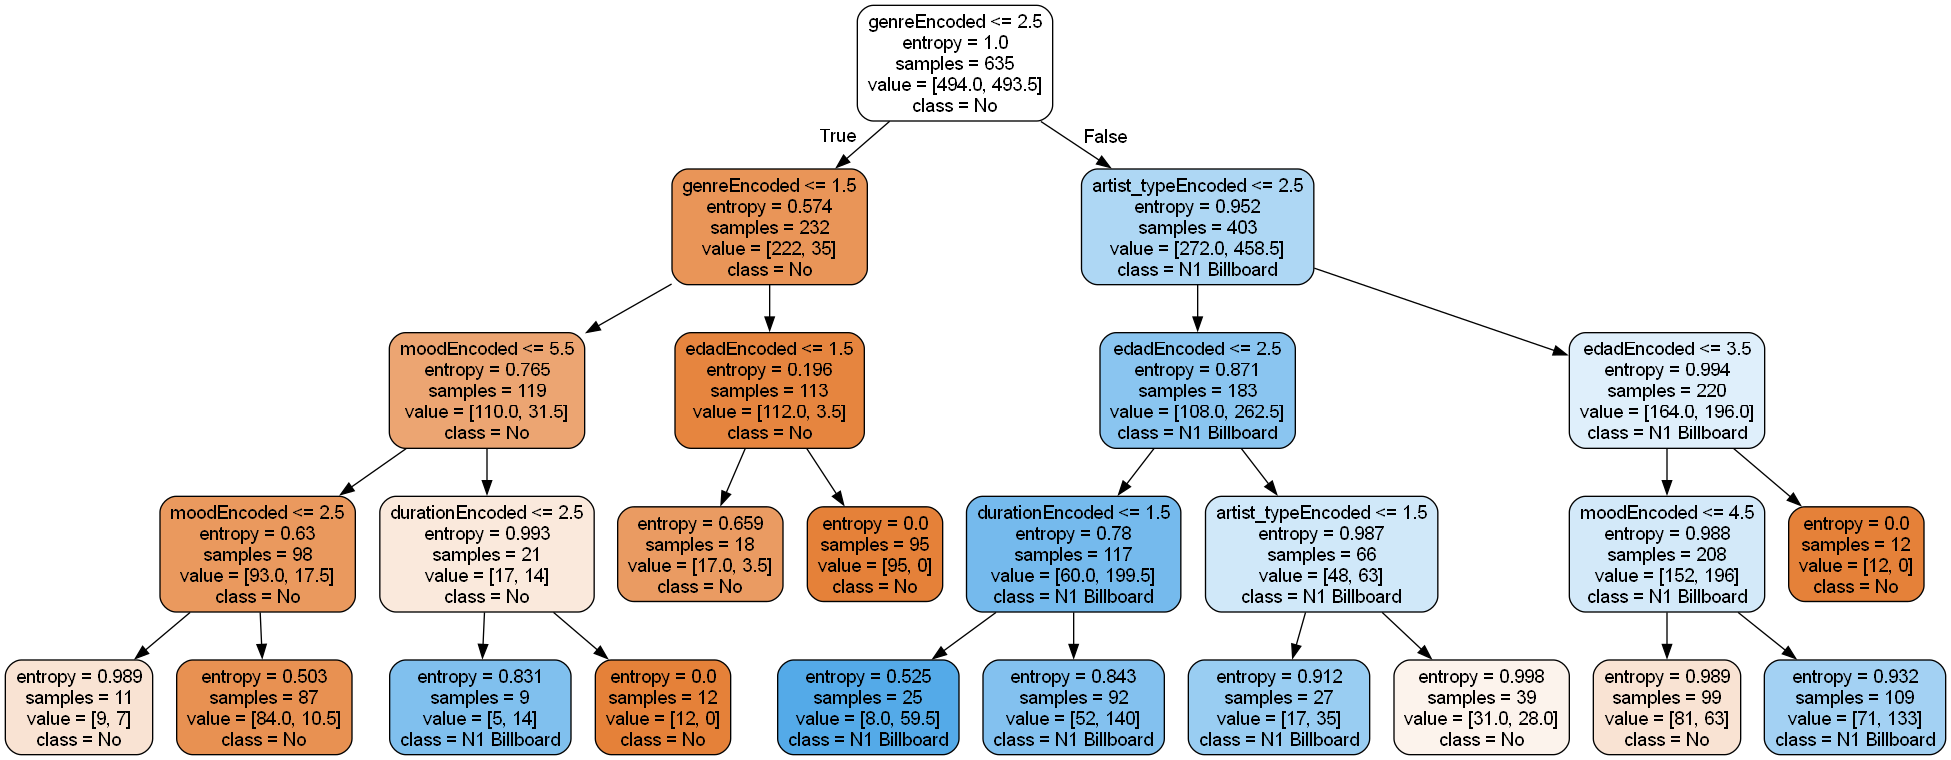
\includegraphics[width=120mm]{tree1.dot.png}
    \caption{The decision tree.}
    \label{fig:tree}
\end{figure}

\section{Results}
We can see in Figure \ref{fig:tree} there are questions that depending on the answer, reduce the entropy by a lot or not. For example, if the genre is not urban or pop (true path for the root node) the entropy is reduced almost by half, which indicated that a lot of top 1 songs are urban or pop. \par
As for predictions, we can predict if the song Havana by Camila Cabello would make it to the top 1 of the billboard chart. The model says that it will with an $86.21\%$ of accuracy, and the model is correct since this song reached top 1 in 2017.

\section{Conclusions}
The decision tree is a very powerful model for classification, but can be a little tricky when working with categorical or continuous variables. As with every model, it works best as the sample gets bigger and does not contain missing data. \par
Since we did a lot of analysis before actually creating the model, the created decision tree became a very trustworthy model for predictions.

\bibliographystyle{../common_styles/cs-agh}
\bibliography{act12_bibliography}

\end{document}